\documentclass[10pt]{article}

\usepackage{spheric}
%%%TITLE
\title{Adaptive particle splitting in the Finite Volume Particle Method}
\date{}

%%AFFILIATIONS
\author[$\relax$]{Nathan J. Quinlan}

\affil[$\relax$]{Mechanical Engineering, National University of Ireland Galway}


%%DOCUMENT
\begin{document}

\maketitle

%\SelectedTopics{}

%%PLEASE PUT YOUR ABSTRACT HERE
\begin{abstract}
The Finite Volume Particle Method (FVPM) is based on overlapping compactly support variable-mass particles (as in ALE-SPH) and employs interparticle area analogous to intercell area in the classical mesh-based finite volume method. It maintains exact conservation and zero-order consistency in non-uniform particle size distribution. This property makes it a strong candidate for implementation of adaptive particle distribution by particle splitting, which has the potential to reduce computational costs by orders of magnitude in complex problems. Adaptive particle splitting has previously been developed in SPH by several authors \cite{lastiwka2005adaptive,barcarolo2014adaptive,lopez2013dynamic} and in FVPM \cite{jahanbakhsh2016development}.

In this paper, particle splitting will be developed for 2D FVPM, with results for various benchmark cases. Square particles are used, with the advantage that a parent may be split into four children which align with its support. It will be shown that volume, mass and momentum can be exactly conserved as a result. Field variables must be interpolated from the parent to the new particles. Analysis will be presented to show that the conservative scheme with minimum error is simply a zero-order interpolation. This introduces a first-order error at the site of splitting, which must be balanced against the reduction in error achieved in regions of refined particles.

Sample results are shown in Figure \ref{fig:12} for the dambreak case described by Barcarolo et al. \cite{lopez2013dynamic}. When a particle approaches the right wall, it is split into 4 new particles of size equal to 0.55 of the parent size. The evolution of kinetic energy is shown for a static coarse particle distribution, a distribution refined by dynamic splitting, and a static fine (hence, expensive) distribution. There is excellent agreement between the results for the static fine distribution and the dynamically refined distribution with splitting. This indicates that splitting enables accuracy to be maintained or enhanced with significant reductions in computational cost.
 
\begin{figure}[!htb]
\begin{minipage}[b]{0.5\linewidth}
\centering
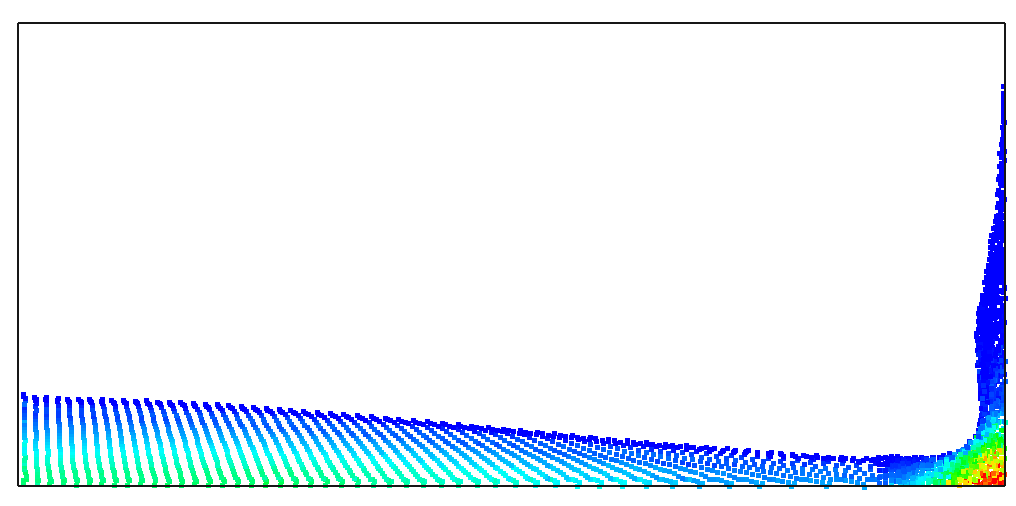
\includegraphics[width=0.7\textwidth]{12-11.png}\\ (a)

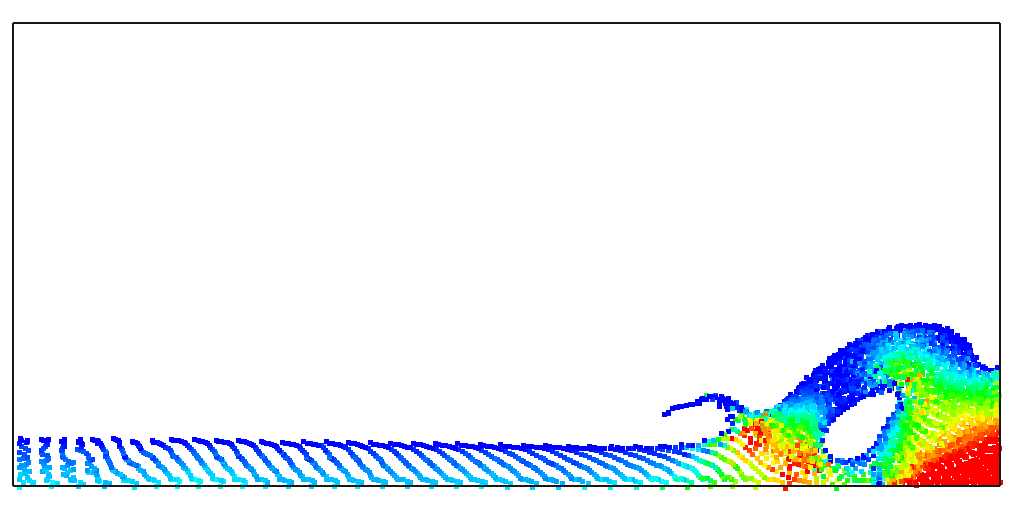
\includegraphics[width=0.7\textwidth]{12-12.png}\\ (b)
\end{minipage}
\begin{minipage}[b]{0.5\linewidth}
\centering
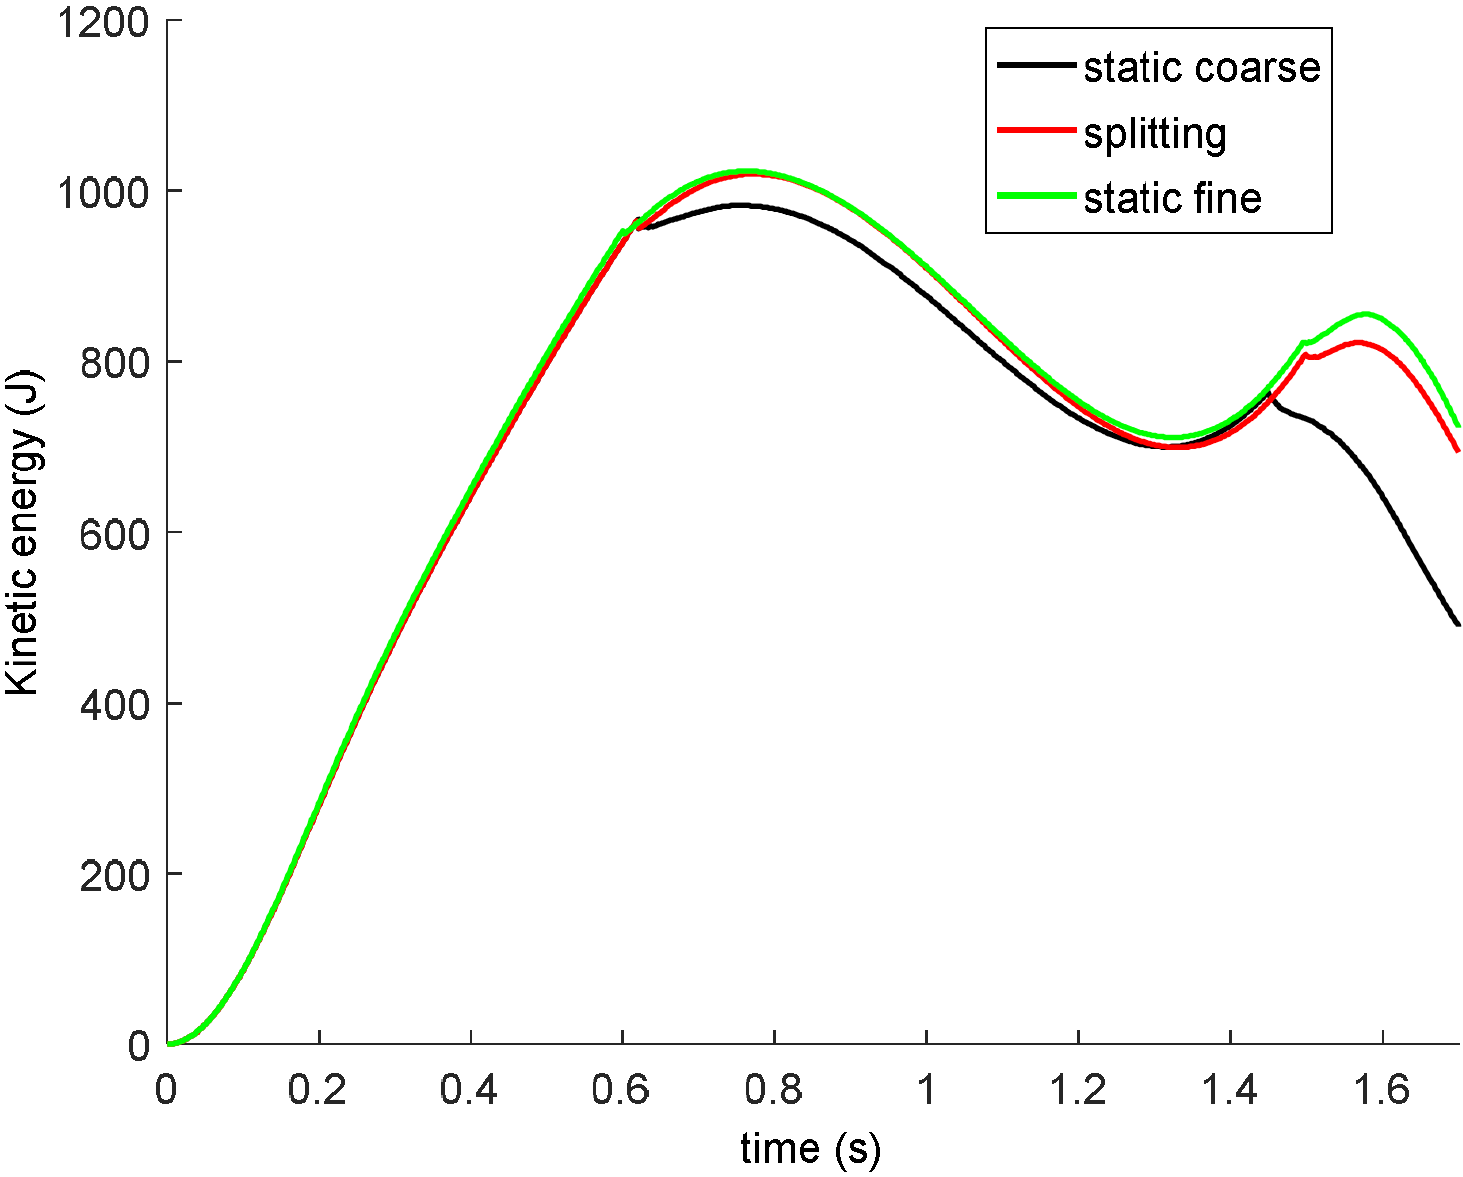
\includegraphics[width=0.95\textwidth]{12-13.png}\\ (c)
\end{minipage}
\caption{(a) and (b) instantaneous pressure fields in the dambreak flow. Particle splitting occurs at the dashed line. (c) Evolution of total
kinetic energy.}\label{fig:12}
\end{figure}




\end{abstract}


%%THE END OF ABSTRACT

\addbib

\end{document}
